\chapter{Conclusions}

The lofty goal set out at the beginning of this thesis was to develop the architecture of a quantum computer. Unfortunately,
as I hope has become clear throughout the course of your reading, reaching the goal of a universal quantum computer
is not yet within our grasp. However, what I have aimed to do here is to have made progress towards a general purpose quantum machine at each
level of the quantum computing stack, from the high level architecture in Chapter~\ref{sec:arch}, to the low level challenges
of designing materials for qubits in Chapter~\ref{sec:majoinas}. As I come to the close of this thesis, I will reflect on the outstanding
challenges of realizing a quantum computer, including on areas where I think there is significant risk.

\section{Controlling Qubits}
At the top of the stack, in Chapter~\ref{sec:arch}, I discussed the challenges of designing quantum devices that can scale up to the large number of
control and readout lines that a useful quantum machine would require. In addition, I presented architectures that lower the
requirements on both the number of dc and rf lines, and on the power dissipation required to control a quantum device. Today, the effort to build
CryoCMOS architectures for controlling qubits has been joined by a number of groups, including Google~\cite{gcryocmos}, Intel and Delft university~\cite{VANDIJK201990}
well and truly in the race to build components for scaleable cryogenic operation of both superconducting and semiconducting qubits. The aims of each
of these efforts is twofold, firstly to bring the footprint of the qubit-classical interface under control, the second being
to tame the growth of power consumption in each part of the stack.

In Sec.~\ref{sec:archdesign}, the requirement for control and readout fidelity was also given alongside the requirements for footprint and power. Pointedly,
these two requirements are not listed with the above, since the reality of the modern quantum physics experiment is that the bulky room temperature readout
and control hardware is largely superior to hardware we build for cryogenic operation. This is not surprising, much of the hardware that is currently used
for readout and control, be it oscilloscopes, network analyzers, vector sources and so forth, trade off power and size for flexibility and performance, which
are unfortunately not what is needed to scale quantum systems. The challenge for each of the architectures listed in Chapter~\ref{sec:arch}, and for those
being developed externally, is to match

\section{Closing Remarks}
The field today is focussed on achieving quantum supremacy, that is to run an algorithm on a quantum computer that could not feasibly be
simulated on a classical machine. The consensus at the time of writing is that this will be some variant of Boson sampling~\cite{Aaronson:2011},
performed on approximately 50 qubits~\cite{savage,8322045,10.1038/s41567-018-0131-y}, with companies such as Google, IBM, Rigetti and Ion-Q each having
announced their intention to reach this goal imminently. However, even though IBM announced its 50 qubit processor in November 2017~\cite{ibmq}, Google announced
its Bristlecone chip containing 72 qubits at the March Meeting of the American Physical Society in 2018~\cite{bristlecone,Neill195} and Intel announced
its 49 qubit quantum processor in January at CES 2018~\cite{intelq}, the goal of quantum supremacy lies tantalizingly just out of reach. From a scientific standpoint,
this is perhaps not surprising. There is plenty of evidence that even for the problem of Boson sampling, the quality of qubits must be higher
than expected~\cite{PhysRevX.6.021039,PhysRevLett.117.080501}, the connectivity of qubits must be relatively high~\cite{s41567-018-0124-x},
and that the number of qubits might be larger than thought~\cite{2017arXiv171005867P}.
From the standpoint of a quantum physicist and engineer, this represents an exciting challenge, one that calls for further incremental improvement of qubits,
for new designs that extend the connectivity of qubits and for improved methods of readout and control. From the perspective of the public and the community, however,
there lies some danger, wherein we run the risk of hitting a "Quantum Winter". This would be a period analogous to the "AI Winter"~\cite{crevier1993ai},
a period in the history of artificial intelligence, where persistent hype and an over-selling of the promise of AI, followed by a failure to deliver on these promises,
led to a period of reduced funding and interest in the field. The reason that quantum supremacy has not yet been achieved may not be surprising to those in the
field, but has regularly been a source of surprise to members of the public.

\begin{figure}
    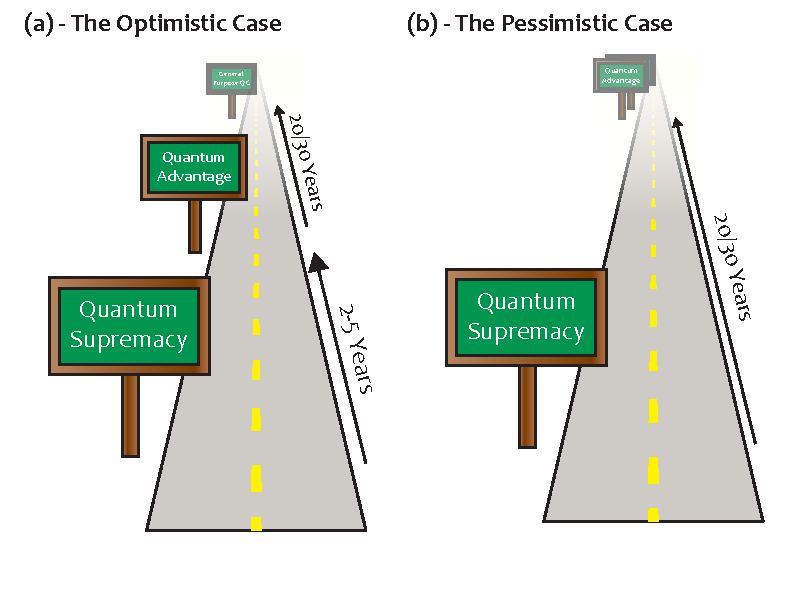
\includegraphics[width=0.7\linewidth]{Roadmap}
    \caption[Roadmap to a quantum computer]{\label{fig:roadmap} The possible paths by which a quantum computer is achieved. (a) In the optimistic case, a few years after
    quantum supremacy is reached, an algorithm demonstrating quantum advantage is achieved, leading to continued interest in the field. (b) In the pessimistic case,
    even though quantum supremacy is reached, the demonstration of an algorithm that shows quantum advantage doesn't occur until a general purpose quantum machine is available.}
\end{figure}

If we assume, however, that we reach the goal of quantum supremacy in the reasonably near future, there are two roadmaps to a general purpose quantum machine, one which
presents great opportunities for quantum computing researchers, the other which presents a risk that we must confront to ensure that development continues sustainably.
These two roadmaps are shown in Fig.~\ref{fig:roadmap}, and relate to the demonstration of quantum advantage, that is the solution of a problem with a quantum computer
that would not have been possible without one. Equivalently, the question is "what is interesting in the NISQ era"~\cite{Preskill2018quantumcomputingin}? In Fig.~\ref{fig:roadmap}
(a), the answer is "something". This may be Variational Quantum Eigensolvers (VQEs)~\cite{nature23879}, it may be some form of machine learning~\cite{PhysRevLett.121.040502},
however there is yet every chance that even these algorithms may turn out to be classically tractable~\cite{Tang:2019:QCA:3313276.3316310,10.1038/nphys3272}, or requires
error correction to the extent that we are pushed to the realm of needing a general purpose quantum machine~\cite{Reiher7555}. In this case, we may live in a world where
Fig.~\ref{fig:roadmap} (b) is true, and there is a long period of time where a quantum computer is simply a toy. Such a situation would require continued long term investment,
and is not a future that we should ignore in our current push to build a quantum computer.

Despite the risk, it is also true that at no other point in the history of quantum computing has there been such great awareness of the magnitude of the problems
that must be solved. There is constant development in all areas of the stack, from proposals for quantum programming languages, to improved equipment for quantum
experiments to even new types of qubit. Together, all of this convinces me that, barring an extraordinary no-go result, a useful quantum computer is not only
achievable, but will be realized in the next 20 or so years. I can't predict the form of such a quantum computer, nor how it will be used, however regardless of
it's final form, it will confer benefits on all of humanity.
